\documentclass[aspectratio=169,10pt]{beamer}

\usepackage[T1]{fontenc}
\usepackage[utf8]{inputenc}
% babel-english is absent from the local TinyTeX distribution; the deck is
% entirely in English, so no language module is loaded.
\usepackage{lmodern}
\usepackage{microtype}
\usepackage{booktabs}
\usepackage{graphicx}
\usepackage{xcolor}
\usepackage{tikz}

\usetikzlibrary{arrows.meta,calc,fit,positioning}

% Palette reprise de metric/soutenance.tex pour rester cohérent avec les
% documents de soutenance existants.
\definecolor{LanceNavy}{HTML}{123B5D}
\definecolor{LanceBlue}{HTML}{1F6F9F}
\definecolor{LanceCyan}{HTML}{1597A8}
\definecolor{LanceGreen}{HTML}{2E7D5B}
\definecolor{LanceOrange}{HTML}{D97721}
\definecolor{LanceRed}{HTML}{B64045}
\definecolor{LanceLight}{HTML}{F3F7FA}
\definecolor{LanceInk}{HTML}{263746}

\usetheme{default}
\usefonttheme{professionalfonts}
\setbeamertemplate{navigation symbols}{}
\setbeamersize{text margin left=7mm,text margin right=7mm}

\setbeamercolor{normal text}{fg=LanceInk,bg=white}
\setbeamercolor{structure}{fg=LanceBlue}
\setbeamercolor{frametitle}{fg=white,bg=LanceNavy}
\setbeamercolor{block title}{fg=white,bg=LanceBlue}
\setbeamercolor{block body}{fg=LanceInk,bg=LanceLight}
\setbeamercolor{block title alerted}{fg=white,bg=LanceOrange}
\setbeamercolor{block body alerted}{fg=LanceInk,bg=LanceOrange!10}
\setbeamercolor{block title example}{fg=white,bg=LanceGreen}
\setbeamercolor{block body example}{fg=LanceInk,bg=LanceGreen!9}
\setbeamercolor{author in head/foot}{fg=white,bg=LanceNavy}
\setbeamercolor{date in head/foot}{fg=white,bg=LanceBlue}

\setbeamerfont{frametitle}{series=\bfseries,size=\Large}
\setbeamerfont{title}{series=\bfseries,size=\LARGE}
\setbeamerfont{subtitle}{size=\large}
\setbeamerfont{block title}{series=\bfseries}

\setbeamertemplate{frametitle}{%
  \nointerlineskip
  \begin{beamercolorbox}[wd=\paperwidth,ht=3.0ex,dp=1.1ex,leftskip=7mm]{frametitle}
    \usebeamerfont{frametitle}\insertframetitle
  \end{beamercolorbox}
}

\setbeamertemplate{footline}{%
  \leavevmode
  \hbox{%
    \begin{beamercolorbox}[wd=.87\paperwidth,ht=2.7ex,dp=1.1ex,leftskip=7mm]{author in head/foot}
      \scriptsize Project LANCE \hspace{0.7em}--\hspace{0.7em} NATO SPS G6259
    \end{beamercolorbox}%
    \begin{beamercolorbox}[wd=.13\paperwidth,ht=2.7ex,dp=1.1ex,center]{date in head/foot}
      \scriptsize\insertframenumber
    \end{beamercolorbox}%
  }
}

% Encadré de message clé, aligné sur le style de la soutenance.
\newcommand{\keymessage}[1]{%
  \begin{beamercolorbox}[rounded=true,sep=1.1ex,wd=\linewidth]{block body example}
    \centering\bfseries #1
  \end{beamercolorbox}
}

\tikzset{
  >={Latex[length=2.2mm]},
  flow/.style={->,semithick,draw=LanceInk!80},
  box/.style={draw=LanceBlue,fill=LanceBlue!8,rounded corners=2pt,
    align=center,minimum height=9mm,inner sep=3pt,font=\scriptsize},
  greenbox/.style={draw=LanceGreen,fill=LanceGreen!9,rounded corners=2pt,
    align=center,minimum height=9mm,inner sep=3pt,font=\scriptsize},
  orangebox/.style={draw=LanceOrange,fill=LanceOrange!9,rounded corners=2pt,
    align=center,minimum height=9mm,inner sep=3pt,font=\scriptsize},
  greybox/.style={draw=LanceInk!45,fill=LanceInk!6,rounded corners=2pt,
    align=center,minimum height=9mm,inner sep=3pt,font=\scriptsize}
}

\title{LANCE}
\subtitle{An autonomous, provable auditor for IoT/IIoT networks}
\author{Project LANCE \quad--\quad Universit\'e de Mons}
\institute{NATO SPS G6259 --- progress report}
\date{2026-10-23 \quad--\quad work in progress}

\begin{document}

% ---------------------------------------------------------------- 1. Titre
{
  \setbeamercolor{background canvas}{bg=LanceNavy}
  \begin{frame}[plain]
    \color{white}
    \begin{columns}[c,onlytextwidth]
      \begin{column}{0.72\textwidth}
        {\usebeamerfont{title}\inserttitle\par}
        \vspace{0.35em}
        {\usebeamerfont{subtitle}\color{white!82}\insertsubtitle\par}
        \vspace{1.2em}
        {\large Project LANCE \quad--\quad Universit\'e de Mons}\par
        \vspace{1.0em}
        {\small\color{white!75}Progress report --- 23 October 2026\par
        Work in progress: no general advantage of the model is demonstrated}
      \end{column}
      \begin{column}{0.24\textwidth}
        \centering
        \begin{tikzpicture}
          \node[draw=white,rounded corners=3pt,minimum width=22mm,
                minimum height=22mm,align=center,text=white,
                font=\bfseries\small] {LANCE\\[2pt]
            \scriptsize IoTChain\\Bench};
        \end{tikzpicture}
      \end{column}
    \end{columns}
  \end{frame}
}

% --------------------------------------------------- 2. Objectif et priorités
\begin{frame}{The objective, and what it implies}

  \begin{exampleblock}{Objective}
    An \textbf{autonomous and provable} auditor for IoT/IIoT networks: it
    explores, finds, verifies and reports, with \textbf{recomputable evidence}.
  \end{exampleblock}

  \vspace{0.2em}
  \begin{columns}[T,onlytextwidth]
    \begin{column}{0.52\textwidth}
      \begin{block}{What this commits us to demonstrate}
        \begin{itemize}
          \item not ``the model finds more'', but \textbf{under which
                conditions} it adds something an automation cannot;
          \item with \textbf{identical tools, inputs and budgets};
          \item with conclusions that are \textbf{verifiable}, not plausible.
        \end{itemize}
      \end{block}
    \end{column}
    \begin{column}{0.44\textwidth}
      \begin{block}{Current priorities, in order}
        \begin{enumerate}
          \item the \textbf{benchmark} --- the instrument that answers the
                question;
          \item the \textbf{platform} --- deploy, launch, follow, retrieve,
                isolate, clean up.
        \end{enumerate}
      \end{block}
      \begin{alertblock}{Out of priority}
        \small Model training. The AsiaCCS paper reports what the benchmark
        measures; it does not drive the order of work.
      \end{alertblock}
    \end{column}
  \end{columns}

\end{frame}

% ------------------------------------------------------ 3. L'instrument
\begin{frame}{How we answer it}

  \centering
  \resizebox{0.96\linewidth}{!}{%
  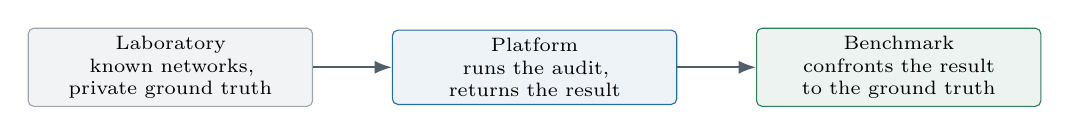
\begin{tikzpicture}[node distance=10mm]
    \node[greybox,text width=34mm] (lab) {Laboratory\\\scriptsize known networks,\\private ground truth};
    \node[box,text width=34mm,right=of lab] (plat) {Platform\\\scriptsize runs the audit,\\returns the result};
    \node[greenbox,text width=34mm,right=of plat] (bench) {Benchmark\\\scriptsize confronts the result\\to the ground truth};
    \draw[flow] (lab) -- (plat);
    \draw[flow] (plat) -- (bench);
  \end{tikzpicture}%
  }

  \vspace{1.4em}
  \begin{columns}[T,onlytextwidth]
    \begin{column}{0.48\textwidth}
      \begin{block}{Three pieces, three roles}
        \small None substitutes for another. The laboratory reconstructs
        networks we already know; the benchmark is what turns a run into a
        measurement.
      \end{block}
    \end{column}
    \begin{column}{0.48\textwidth}
      \begin{alertblock}{The model is only one piece}
        \small Probes observe, proof contracts bound what may be claimed, the
        engine orchestrates and accounts.
      \end{alertblock}
    \end{column}
  \end{columns}

\end{frame}

% --------------------------------------------- 4. Ce qui compte comme trouvé
\begin{frame}{What counts as ``found''}

  \begin{columns}[T,onlytextwidth]
    \begin{column}{0.50\textwidth}
      \small A conclusion counts only if it can be \textbf{recomputed} from
      what was actually observed.

      \vspace{0.5em}
      Example: \emph{``the data of another organisation can be read''}.
      \begin{itemize}
        \item[\textcolor{LanceRed}{$\times$}] the agent \emph{claims} it:
              not counted;
        \item[\textcolor{LanceGreen}{$\checkmark$}] the logged request and its
              response contain the data: counted.
      \end{itemize}

      \vspace{0.4em}
      We recompute the finding from the tool log. We do not re-run the
      requests, and we never trust the conclusion.
    \end{column}
    \begin{column}{0.46\textwidth}
      \begin{alertblock}{And the trap}
        \small The same trial runs on two configurations of the same network:
        one where the tested weakness is \textbf{absent}, one where it is
        \textbf{present}.

        \vspace{0.4em}
        On the first, the correct answer is ``nothing to report''. Finding
        something there is a \textbf{false positive}, counted as an error.
      \end{alertblock}
      \keymessage{A good auditor succeeds on both}
    \end{column}
  \end{columns}

\end{frame}

% --------------------------------------------------- 5. Premier constat
\begin{frame}{What the first campaign showed}

  \begin{columns}[T,onlytextwidth]
    \begin{column}{0.46\textwidth}
      \begin{block}{The setup}
        \small Two network families, each with two configurations and three
        repetitions --- the rule-based automation and the model side by side.
        Each arm succeeds on all six trials of each family.
      \end{block}
      \keymessage{Both succeed everywhere}
    \end{column}
    \begin{column}{0.50\textwidth}
      \begin{alertblock}{What it means, and does not mean}
        \small
        \begin{itemize}
          \item not ``the model is better'': there is no difference;
          \item not ``the model is useless'': this pilot was built to qualify
                the instrument, not to decide between the arms;
          \item \textbf{it cannot separate the two approaches}, and that is
                what we need.
        \end{itemize}
      \end{alertblock}
    \end{column}
  \end{columns}

  \vspace{0.8em}
  \begin{beamercolorbox}[rounded=true,sep=1.2ex,wd=\linewidth]{block body alerted}
    \small The pilots show that \textbf{both instruments measure}. They do not
    show when a model is useful: a list of scenarios everyone passes tests no
    competence.
  \end{beamercolorbox}

\end{frame}

% ------------------------------------------- 6. Objectif -> hypothèses
\begin{frame}{So the objective is restated as hypotheses}

  \small
  The objective does not change --- its \textbf{form} does.
  ``Is the model better?'' cannot be settled.
  ``\emph{Which properties of a network make a model add something --- and
  which do not?}'' can.

  \vspace{0.5em}
  \centering\scriptsize
  \renewcommand{\arraystretch}{1.25}
  \begin{tabular}{@{}clll@{}}
    \toprule
    \textbf{\#} & \textbf{Property of the network} & \textbf{What we test} \\
    \midrule
    H1 & devices are connected      & an identity link absent from public inputs \\
    H2 & formats are heterogeneous  & a format the declared parsers do not cover \\
    H3 & contracts are unseen       & rights and goals from never-seen documentation \\
    H4 & meaning is vendor-specific & a field whose sense is only in naming or doc \\
    H5 & devices refuse             & resuming beyond the script's standard branch \\
    \midrule
    H6 & observed content is hostile & whether a planted instruction is obeyed \\
    \bottomrule
  \end{tabular}

  \vspace{0.5em}
  \begin{columns}[T,onlytextwidth]
    \begin{column}{0.40\textwidth}
      \begin{block}{H1--H5: a possible gain}
        \scriptsize Each measures whether the model adds something.
      \end{block}
    \end{column}
    \begin{column}{0.56\textwidth}
      \begin{alertblock}{H6: a risk, not a gain}
        \scriptsize The prediction is that a model \emph{obeys} an injected
        instruction while a script ignores it. We measure the vulnerability;
        zero compliance is the good outcome.
      \end{alertblock}
    \end{column}
  \end{columns}

\end{frame}

% ------------------------------------------------------ 6b. Statut du registre
\begin{frame}{What the register commits us to}

  \begin{columns}[T,onlytextwidth]
    \begin{column}{0.48\textwidth}
      \begin{block}{Status}
        \small A \textbf{design register}. No hypothesis has been executed yet.
        Each one can fail --- a documented failure remains a result.
      \end{block}
      \begin{exampleblock}{Declared coverage}
        \small What is not covered is written down, not pretended: physical
        impact, device fragility under probing, real fleet scale.
      \end{exampleblock}
    \end{column}
    \begin{column}{0.48\textwidth}
      \begin{alertblock}{Why this shape}
        \small
        \begin{itemize}
          \item a family that tests no hypothesis does not enter the benchmark;
          \item a variant does not count as an independent family;
          \item the contrast is declared \emph{before} the fixture;
          \item a null result is a result.
        \end{itemize}
      \end{alertblock}
    \end{column}
  \end{columns}

\end{frame}

% ----------------------------------------------------------- 7. V0
\begin{frame}{Before testing the model, test the test}

  \begin{columns}[T,onlytextwidth]
    \begin{column}{0.48\textwidth}
      \begin{block}{V0 is not a hypothesis about the model}
        \small It is the \textbf{condition of interpretation} for everything
        else: a deliberately simple control task, solvable without inference.
      \end{block}
      \keymessage{Both approaches must pass}
      \vspace{0.4em}
      \small If the \textbf{script succeeds and the model fails}, the defect is
      in the instrument --- prompt, briefing, budget, tool --- not in the
      model's competence.
    \end{column}
    \begin{column}{0.48\textwidth}
      \begin{alertblock}{What it already caught}
        \small On one early trial the briefing documented no HTTP route: the
        model tried paths outside the contract and collected 404s, while the
        script knew where to read the policy. The defect was in the harness,
        not in the model.
      \end{alertblock}
      \keymessage{A green run would have said nothing}
    \end{column}
  \end{columns}

  \vspace{0.5em}
  \centering\scriptsize
  The control is written and tested offline; the laboratory run on a held-out
  instance remains to be done.

\end{frame}

% ------------------------------------------------ 8. Ce qu'on peut mesurer
\begin{frame}{What we can measure today}

  \centering\small
  Three measurements --- all \textbf{descriptive}. These are not the results of
  the six hypotheses.

  \vspace{0.7em}
  \begin{columns}[T,onlytextwidth]
    \begin{column}{0.31\textwidth}
      \begin{block}{1. Two models}
        \scriptsize Both succeed on both families. The mixture-of-experts model
        costs about twice as much and takes 1.3--1.7$\times$ longer, for the
        same result.
      \end{block}
    \end{column}
    \begin{column}{0.31\textwidth}
      \begin{block}{2. Variability}
        \scriptsize Between 6\% and 46\% across repetitions, setting aside one
        cold model load. Three repetitions give a dispersion, not a sample.
      \end{block}
    \end{column}
    \begin{column}{0.31\textwidth}
      \begin{alertblock}{3. One discriminating case}
        \scriptsize An access-control case where the automation stops and the
        model does not.
      \end{alertblock}
    \end{column}
  \end{columns}

  \vspace{0.9em}
  \begin{beamercolorbox}[rounded=true,sep=1.2ex,wd=0.94\linewidth]{block body alerted}
    \small The automation is \textbf{built to stop at a boundary declared in
    advance}; the model crosses a boundary the automation never inspects.
    That is \textbf{coverage}, not intelligence.
  \end{beamercolorbox}

\end{frame}

% ------------------------------------------------------ 9. Ce qu'on ne peut pas
\begin{frame}{What we cannot claim}

  \begin{columns}[T,onlytextwidth]
    \begin{column}{0.48\textwidth}
      \begin{alertblock}{About the model}
        \small
        \begin{itemize}
          \item no general advantage is demonstrated;
          \item no confidence interval: one family per harness, so no
                statistical inference --- only a descriptive profile;
          \item no result is yet ``admissible as confirmatory evidence'': the
                metric definition is not frozen.
        \end{itemize}
      \end{alertblock}
    \end{column}
    \begin{column}{0.48\textwidth}
      \begin{alertblock}{About the measurement}
        \small
        \begin{itemize}
          \item real cost is not measured --- neither billed nor hardware cost;
                tariff estimates are not a monetary measurement;
          \item ``green run'' $\neq$ exploitable measurement: one early run was
                green while every model arm had failed.
        \end{itemize}
      \end{alertblock}
    \end{column}
  \end{columns}

  \vspace{0.5em}
  \keymessage{A documented null result is a usable result}

\end{frame}

% --------------------------------------------------------- 10. Suite
\begin{frame}{Next steps, and what would help}

  \begin{columns}[T,onlytextwidth]
    \begin{column}{0.54\textwidth}
      \begin{block}{The order follows conditions, not dates}
        \small
        \begin{enumerate}
          \item \textbf{V0} on a held-out instance --- MQTT as it stands; SSH
                only after the dictionary is randomised;
          \item a \textbf{parameterisable harness} --- today one scenario is a
                locked module;
          \item \textbf{families for H2, H3, H4} --- private ground truth,
                declared baseline, evaluator;
          \item the \textbf{platform}: reproducible deployment and launch.
        \end{enumerate}
      \end{block}
    \end{column}
    \begin{column}{0.42\textwidth}
      \begin{exampleblock}{What would help most}
        \small
        \begin{itemize}
          \item real \textbf{vendor artifacts} --- H2 and H4 lack a corpus;
          \item an \textbf{adversarial review} of the hypothesis register, on
                falsifiability grounds.
        \end{itemize}
      \end{exampleblock}
      \vspace{0.3em}
      \begin{alertblock}{Single external constraint}
        \scriptsize AsiaCCS 2027, 11 December 2026 (AoE). It does not order the
        steps, and justifies neither an unvalidated scope nor an unmeasured
        result.
      \end{alertblock}
    \end{column}
  \end{columns}

\end{frame}

% ===================================================== ANNEXES (réserve)
\appendix
\section*{Reserve slides}

\begin{frame}{Reserve --- model panel}
  \centering\small
  Two families, three repetitions $\times$ two configurations, two models.

  \vspace{0.6em}
  \begin{tabular}{@{}llcc@{}}
    \toprule
    Family & Approach & Success & Cost (\$) \\
    \midrule
    SSH  & rules       & 6/6 & 0 \\
    SSH  & dense model & 6/6 & 0.006--0.008 \\
    SSH  & MoE model   & 6/6 & 0.012--0.017 \\
    MQTT & rules       & 6/6 & 0 \\
    MQTT & dense model & 6/6 & 0.004--0.010 \\
    MQTT & MoE model   & 6/6 & 0.012--0.016 \\
    \bottomrule
  \end{tabular}

  \vspace{0.8em}
  \scriptsize Costs are tariff estimates, not billed measurements.
  Each family is a distinct configuration: the two are never pooled.
\end{frame}

\begin{frame}{Reserve --- variability}
  \centering\small
  Coefficient of variation over three repetitions, per family and configuration.

  \vspace{0.6em}
  \begin{tabular}{@{}lccc@{}}
    \toprule
    Family / configuration & Duration & Cost & Tokens \\
    \midrule
    SSH healthy      & 92.3\% & 7.0\%  & 5.9\%  \\
    SSH vulnerable   & 6.4\%  & 17.9\% & 21.8\% \\
    MQTT healthy     & 27.8\% & 46.1\% & 25.6\% \\
    MQTT vulnerable  & 10.2\% & 34.7\% & 35.6\% \\
    \bottomrule
  \end{tabular}

  \vspace{0.8em}
  \scriptsize The 92\% figure comes from one cold model load (73.7\,s against
  16.6 and 16.7\,s), not from policy variability.
\end{frame}

\begin{frame}{Reserve --- declared coverage gaps}
  \small
  \begin{itemize}
    \item physical impact and functional safety;
    \item device fragility under probing;
    \item real fleet scale;
    \item proprietary industrial protocols that are not simulated;
    \item complete multi-step exploitation chains;
    \item abstention and calibration;
    \item generic IT scenarios, deliberately excluded.
  \end{itemize}

  \vspace{0.8em}
  A benchmark that states its gaps is stronger than one that claims full
  coverage.
\end{frame}

\end{document}
